\documentclass[a4paper]{article}
\usepackage{fancyhdr}
\usepackage{amsmath}
\usepackage{xcolor}
\usepackage{graphicx}
\usepackage{latexsym}
\usepackage{amssymb}
\usepackage{listings}

\lstset{basicstyle=\footnotesize,breaklines=true}

%%clickable links
\usepackage{hyperref}
\hypersetup{
    colorlinks=true, %colore les liens
    breaklinks=true, %permet le retour à la ligne dans les liens trop longs
    urlcolor= blue, %couleur des hyperliens
    linkcolor= black, %couleur des liens internes
}
%formatted algorithm:
\usepackage{algpseudocode}
\usepackage{algorithm}

\algblockdefx[Event]{Event}{EndEvent}%
[1][]{\textbf{Upon event :} #1}%
{}

\algblockdefx[Data]{Data}{EndData}%
[1][]{\textbf{Data :}}%
{}


\algblockdefx[Init]{Init}{EndInit}%
[1][]{\textbf{Initialization :}}%
{}


%% New commands
\newcommand{\eqdef}{\;\stackrel{\text{def}}{=}\;}

\begin{document}
\title{Distributed Systems: Network Simulator}
\author{David Benamine \& Rodolphe Lepigre\\
        MOSIG - Parallel, Distributed and Embedded Systems}
\date{\today}
\maketitle

%%%%%%%%%%%%%%%%%%%%%%%%%%%%%%%%%%%%%%%%%%%%%%%%%%%%%%%%%%%%%%%%%%%%%%%%%%%%%%
\section*{Introduction}
As part of our Distributed Network class, we had to build a network simulator
tool and use it to implement and experiment with various broadcast protocols.
In particular we paid much attention to the latency and throughput offered by
the considered protocols.

This report and the source files of the project are both part of our answer to
the problem. The source files should be globally well documented, but reading
this report should help the reader to better understand the structure of the
program.\\

\noindent\textbf{Structure of the report:} In the first section we present the
architecture and functionalities of our simulator. We also present the results
of some tests that we performed to check the behaviour of the system using the
broadcast protocols seen in class (Basic, Tree and Pipe-line broadcast).

In the second and third sections we present two regular total-order broadcast
protocols. The first one achieves a good latency (time for a broadcast to be
achieved with only one process sending), and the second one has a good
throughput when all process are sending at the same time. We also give a
detailed theoretical analysis of the two protocols.

%%%%%%%%%%%%%%%%%%%%%%%%%%%%%%%%%%%%%%%%%%%%%%%%%%%%%%%%%%%%%%%%%%%%%%%%%%%%%%
\section{The network simulator}
In this section we describe the architecture of the network simulator that we
programmed using the C programming language. The simulator follows a round
based approach and makes use of only one thread, as was part of its
specification.

\subsection{Basic principle and usage}
Before diving into a detailed description of the architecture of the program,
we will start by giving some hints on how to use the simulator, and also try
to provide some intuition to the reader on its basic working principles.

Let us first outline some useful terminology that we will use throughout this
report. In our simulator, a single machine capable of sending a message to
other machines will be called a \textit{process}, a \textit{node}, or simply
a \textit{machine}. The term \textit{external event} will refer to any action
taken by the user of the simulator. For example, at some point the user might
decide that a node should initiate a broadcast. This information will be
passed using an external event.

Before being able to use the simulator, the user should first compile it. A
\textit{makefile} is provided in the source directory \textit{src/}. It is
considered that the user is runing a \textit{POSIX}-friendly operating system
and that the regular building tools are present on his machine (\textit{gcc},
\textit{make},...).
\begin{lstlisting}
> cd src/
> make
\end{lstlisting}

Once the program has been (successfully) compiled, an executable file should
have appeared in the source directory. The program contains a ``help'' section
which can be accessed in a standard manner.
\begin{lstlisting}
> ./Broadcast -h
Usage: ../src/Broadcast [-N n][-R n][-h][-b|t|i|p]
Possible arguments:
	-N n	Specify a number of nodes n, default is 4.
	-R n	Specify a number of rounds n, default is 20.
	-h	Display this help message.
Selection of broadcast mode:
	-i	IP broadcast (default).
	-b	Basic broadcast.
	-t	Tree broadcast.
	-p	Pipeline broadcast.
	-L	Total order broadcast with good latency.
	-T	Total order broadcast with good throughput.
\end{lstlisting}

The behaviour of the program can be changed using the command line arguments
as hinted by the ``help'' section content. In particular, the number of nodes
used during the simulation can be set. Also the number of rounds to run can be
set, and if it is set to $0$ the system will run forever.

The broadcast protocol that is going to be used can be selected as well from
the command line. The available options are the following.
\begin{itemize}
  \item IP broadcast: use multicast.
  \item Basic broadcast: the broadcaster sends to every other node in turn
        (one per round).
  \item Pipeline broadcast: the broadcaster sends the message to its neighbour
        which sends it to its neighbour and so on.
  \item Total order broadcast with good latency (described latter).
  \item Total order broadcast with good throughput (described latter).
\end{itemize}

Once the program is run, the simulation starts right away. At each turn, the
user will be prompted to enter external events for the system. Any number of
external event can be entered at the begining of each round. External read on
the standard input (on by line). And when the user is done sending events, he
simply types ``start'' for the simulator to do a round. THe format for the
external events is
\begin{lstlisting}
id event
\end{lstlisting}
where ``id'' is an integer which is the identifier of the node to which the
event is destinated. ``event'' is the content of the event which can be an
arbitrary string (with no line break).
% TODO Give the events that are built-in

\subsection{Architecture of the system}
In order to better understand how the source code is organized, we give a
brief description of the content of every source file.
\begin{itemize}
  \item \textit{Fifo.h} contains a small library providing queues. These are
        used to store pending messages of external events for each process.
        It seems fair for messages (resp. external events) to be sent (resp.
        treated) in the order they arrived in the system (FIFO order: First
        In, First Out).
  \item \textit{Fifo.c} implements the functions defined in \textit{Fifo.h}.
  \item \textit{Message.h} defines what messages (a sender, a receiver and the
        content) and provides functions to initialize, delete and copy
        messages.
  \item \textit{Message.c} implements the functions defined in
        \textit{Message.h}.
  \item \textit{Broadcast.h} contains a definition of the different broadcast
        protocols.
  \item \textit{Broadcast.c} implements all the different broadcast protocols.
  \item \textit{Simulator.h} defines the core functions and data structures
        of the simulator. In particular the function \textit{LaunchSimulation}
        is the core function of the simulator and contains the main loop which
        will do the rounds, read external events and apply the broadcast
        policies defined in \textit{Broadcast.h}.
  \item \textit{Simulator.c} implement the functions defined in
        \textit{Simulator.h}.
  \item \textit{Main.c} contains the main function of the program. It takes
        care of the command line arguments, initialize the system and call
        the \textit{LaunchSimulation} function.
\end{itemize}
% TODO Explain how node functions work and detail what LaunchSimulation does

%%%%%%%%%%%%%%%%%%%%%%%%%%%%%%%%%%%%%%%%%%%%%%%%%%%%%%%%%%%%%%%%%%%%%%%%%%%%%%
\section{A regular total-order broadcast protocols with good latency}
% TODO

\subsection{Description of the protocol}
% TODO

\subsection{Theoretical analysis}
% TODO

\subsubsection*{Latency}
% TODO

\subsubsection*{Throughput}
% TODO

\subsection{Empirical analysis}
% TODO

\subsubsection*{Latency}
% TODO

\subsubsection*{Throughput}
% TODO

%%%%%%%%%%%%%%%%%%%%%%%%%%%%%%%%%%%%%%%%%%%%%%%%%%%%%%%%%%%%%%%%%%%%%%%%%%%%%%
\section{A regular total-order broadcast protocols with good throughput}
This protocol is based on the pipeline broadcast protocol but as soon as a node
receives a message, it will add it to a sorted list. A node $p$ can only deliver the
first message of its list if this message have been acknowledged by the
successor of $p$ in the pipeline or if $p$ is the last node of the pipeline.
This acknowledgement system ensure the total order property (see section
\ref{sec:pipelineack-proof}).

\subsection{Description of the protocol}
\begin{algorithm}[H]
    \centering
    \begin{algorithmic}[5]
        \Data
        \State int : clk
        \Comment{A logical clock}
        \State int : next
        \Comment{the id of the next process in the pipeline}
        \State int : prec
        \Comment{the id of the previous process in the pipeline}
        \State Pending : OrderedList
        \Comment{A list ordered by clock and id}
        \EndData
        \Init
        \State clk$\gets$0
        \State next$\gets$Id()+1\%NProcess
        \If{Id()=0}
        \State prec$\gets$NProcess
        \Else
        \State prec$\gets$Id()-1
        \EndIf
        \State Pending$\gets$EmptyQueue
        \EndInit
        \Event $< tob,Broadcast\ |\ m> $
        \Comment{Start a broadcast}
        \State clk++;
        \State Pending$\rightarrow$add($<m,Id(), clk, false>$) 
        \Comment{The message is added\\}
        \Comment{to the list the false boolean\\}
        \Comment{indicate that we have to wait for one ack}
        \State Send(next,$<m,Id(),clk>$)
        \EndEvent
        \Event $<Receive\ | <m,sender, mclk>>$
        \State clk$\gets$MAX(clk, mclk)+1
        \If{next=sender}
        \State Pending$\rightarrow$add($<m,sender,mclk,true>$)
        \Comment{We are at the end of the pipeline}
        \If{Pending$\rightarrow$IsHead(sender,mclk)}
        \State Pending$\rightarrow$RemoveHead()
        \State Send(prec,$<ack,sender,mclk>$)
        \Comment{m is the first message of\\}
        \Comment{the queue, we can acknowledge it}
        \State Deliver(sender,m)
        \Comment{And deliver it}
        \EndIf
        \Else
        \State Pending$\rightarrow$add($<m,sender,mclk,false>$)
        \State Send(next,$<m,sender,mclk>$)
        \Comment{We forward m through the pipeline}
        \EndIf
        \EndEvent
        \algstore{myalg}
    \end{algorithmic}
    \caption{Pipeline based total ordered broadcast protocol}
\end{algorithm}
\begin{algorithm}[H]
    \centering
    \begin{algorithmic}[5]
        \algrestore{myalg}

        \Event $<Receive\  | <ack,sender, mclk>>$
        \State clk$\gets$ Max(clk,mlck)+1
        \If{Pending$\rightarrow$IsHead(sender,mclk)}
        \Comment{m is the head\\}
        \Comment{we can deliver it}
        \State m$gets$(Pending$\rightarrow$RemoveHead())
        \State Deliver(sender,m)
        \If{sender$\neq$ Id()}
        \Comment{We have to forward the ack}
        \State Send(prec,$<ack,sender,mclk>$
        \EndIf
        \State $<m,sender,mclk,b>\gets$Pending$\rightarrow$getHead()
        \While{b}
        \Comment{While we have receive an ack for\\}
        \Comment{the message at the head of the queue\\}
        \Comment{we can deliver it and forward the ack}
        \State Pending$\rightarrow$RemoveHead()
        \State Deliver(sender,m)
        \If{sender$\neq$ Id()}
        \Comment{We have to forward the ack}
        \State Send(prec,$<ack,sender,mclk>$
        \EndIf
        \State $<m,sender,mclk,b>\gets$(Pending$\rightarrow$getHead())
        \EndWhile
        \Else
        \Comment{m isn't the head we mark m as acknowledged\\}
        \Comment{but we won't forward the ack and deliver it\\}
        \Comment{until m is the head of the pending queue}
        \State Pending$\rightarrow$Remove($<m,sender,mclk,false>$)
        \State Pending$\rightarrow$Add($<m,sender,mclk,true>$)
        \EndIf
        \EndEvent
    \end{algorithmic}
\end{algorithm}
% TODO

\subsection{Theoretical analysis}
% \subsubsection{Proof}
\begin{itemize}
    \item Validity : As there  is no crashes, if a process P broadcast a
        message m, m will be received by every process. If the last
        process haven't any message in it's queue, he will acknowledge
        and deliver m. 
\end{itemize}
\label{sec:pipelineack-proof}

% TODO

\subsubsection*{Latency}
% TODO

\subsubsection*{Throughput}
% TODO

\subsection{Empirical analysis}
% TODO

\subsubsection*{Latency}
% TODO

\subsubsection*{Throughput}
% TODO

%%%%%%%%%%%%%%%%%%%%%%%%%%%%%%%%%%%%%%%%%%%%%%%%%%%%%%%%%%%%%%%%%%%%%%%%%%%%%%
\section*{Conclusion}
% TODO

\end{document}


%%%% Tasks
% Task 1: Design a network simulator
%   * Single thread
%   * Round based
%   * Any programming language
%   * N processes (machines)
%   * No crash
%   * Each machine sends (up to) one message at the begining of a round
%   * Each machine can receive (up to) one message at the end of a round
%
% Task 2: Check the behaviour of the simulator using the broadcast protocols
%         from the lectures.
%   * Basic (Latency = 3, Throughput = 1/3)
%   * Trees (Latency = 2, Throughput = 1/2)
%   * Pipe-line (Latency = 3, Throughput = 1)
%
% Tack 3: Design / Implement two regular total-order broadcast protocols
%   * Assumptions: No crash, perfect link, infinite memory, perfect failure
%                  detector
%   * First protocol: good latency
%   * Second protocol: good throughput (with N senders)
%
% Task 4: Write a report (10 to 15 pages)
%   * Description of simulator architecture
%   * Description of the two protocols
%   * Theoretical analysis of the two protocols (latency, throughput)
%   * Empirical evaluation of the two protocols (using the simulator)


%%%% Some ideas for the protocols

\section*{Protocol for good latency}
\begin{itemize}
    \item Optimized for latency
    \item Bad throughput
    \item Every broadcast go through the same tree
    \item $P_0$ is always the broadcast initiator
    \item $P_0$ is responsible for the order
    \item if $P_i$ want to send a message, he sent it to 0 who do the broadcast
    \item Latency : log(N) + 1 (send to 0)
    \item Throughput : todo
\end{itemize}
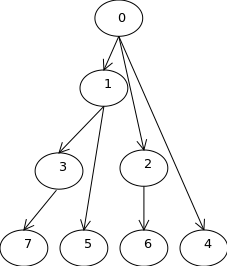
\includegraphics[width=0.5\textwidth]{latencyTO.png}

